\documentclass [10pt] {beamer}
\usetheme      {Madrid}
\usecolortheme {rose}
\usefonttheme  {serif}

\setbeamertemplate {navigation symbols} {}
\setbeamertemplate {footline} [page number]
\setbeamertemplate {caption} [numbered]
\setbeamertemplate {itemize items} [circle]
\setbeamertemplate {enumerate items} [square]
\setbeamertemplate {theorems} [numbered]

\setbeamercolor {footnote mark} {fg = red}
\setbeamercolor {block title} {fg=black}

\setbeamersize {text margin left=10pt, text margin right=10pt}

\usepackage [T2A] {fontenc}
\usepackage [utf8] {inputenc}
\usepackage [english, russian] {babel}
\usepackage {mathrsfs}
\usepackage {graphicx}
\usepackage {ulem}
\usepackage {amssymb}
\usepackage {amsmath}
\usepackage {amsfonts}
\usepackage {indentfirst}
\usepackage {array}
\usepackage {multicol}

\definecolor {forestgreen}   {rgb} {0.13, 0.55, 0.13}
\definecolor {fireenginered} {rgb} {0.81, 0.09, 0.13}
\definecolor {ceruleanblue}  {rgb} {0.16, 0.32, 0.75}

\newtheorem{proposition}{Предложение}

\newcommand{\qu}{\scalebox{1.25}{\bf {\color{ceruleanblue} ?}}}

% \def\redlozenge{\mathbin{\color{red}\blacklozenge}}
% \begin{equation} ... \tag{$\redlozenge$} \end{equation}

\title{Пространственно локализованные решения уравнения Гросса--Питаевского с периодически модулированной нелинейностью}

\author{Лебедев Михаил Евгеньевич}
\institute{
	Институт математики с вычислительным центром \\ УФИЦ РАН \\
	\medskip
	\textit{gloriouslair@gmail.com}
}
\date{Москва -- 2020}

\begin{document}

% ************
% * SLIDE 01 *
% ************
\begin{frame}
	\titlepage
\end{frame}

% ************
% * SLIDE 02 *
% ************
\begin{frame}
	\frametitle{Актуальность работы}

	\begin{multicols}{2}
	[
	Одномерное уравнение Гросса--Питаевского (УГП):
	\begin{equation}
		i \Psi_t + \Psi_{xx} - U(x) \Psi + P(x) |\Psi|^2 \Psi = 0, \quad U(x), P(x) \in \mathbb{R}.
		\label{eq:initial}
	\end{equation}
	В контексте теории конденсата Бозе--Эйнштейна (БЭК) описывает поведение ``сигарообразного'' конденсата; $\Psi(t, x)$ --- {\it \color{ceruleanblue} волновая функция}.
	]
	
	\begin{small}	
	\begin{itemize}
		\setlength\itemsep{5pt}
		\item БЭК --- это состояние вещества, возникающее при сверхнизких температурах.
		\item Предсказан в 1924 году в работах А. Эйнштейна и С. Бозе.
		\item Обнаружен в 1995 году в экспериментах Э. Корнелла, К. Вимана.
		\item 1995--2000-е: эксперименты с различными {\it \color{ceruleanblue} потенциалами удержания} $U(x)$, при этом $P(x) \equiv \pm 1$ (притяжение / отталкивание частиц).
		\item 2000--2010-е: появляются экспериментальные возможности генерации {\it \color{ceruleanblue} периодического псевдопотенциала} $P(x)$.
	\end{itemize}
	\end{small}
	\begin{figure}
		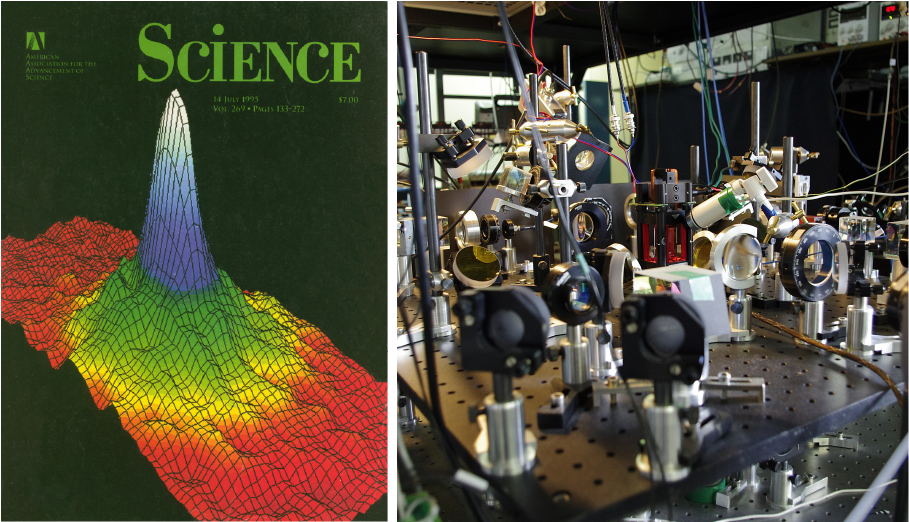
\includegraphics[scale=0.35]{pic/condensate.png}
	\end{figure}
	\end{multicols}
\end{frame}

% ************
% * SLIDE 03 *
% ************
\begin{frame}
	\frametitle{Объект исследования}

	\begin{block}{Стационарные локализованные решения}
	 	Решение уравнения \eqref{eq:initial} называется {\it \color{ceruleanblue} стационарным}, если оно представимо в виде
	 	\begin{equation}
			\Psi(t, x) = u(x) e^{-i \omega t}.	 		
	 	\end{equation}
		Стационарное УГП имеет вид неавтономного уравнения Дюффинга:
		\begin{equation}
			u_{xx} + Q(x) u + P(x) u^3 = 0, \quad Q(x) = \omega - U(x).
			\label{eq:stationary}
		\end{equation}
		Стационарное решение называется {\it \color{ceruleanblue} локализованным}, если $\lim \limits_{x \to \pm \infty} u(x) = 0$.
	\end{block}

	\medskip

	\begin{block}{Регулярные и сингулярные решения}
		Решение уравнения \eqref{eq:stationary} называется {\it \color{ceruleanblue} сингулярным}, если $\exists x_0, \lim \limits_{x \to x_0} u(x) = \infty$.
		Решение, не являющееся сингулярным, называется {\it \color{ceruleanblue} регулярным}.
	\end{block}
\end{frame}

% ************
% * SLIDE 04 *
% ************
\begin{frame}
	\frametitle{Известные результаты}
	
	\begin{small}
	\begin{enumerate}
		\setlength\itemsep{5pt}
		\item[1.] Y. V. Kartashov, B. A. Malomed, L. Torner, Solitons in nonlinear lattices // Rev. Mod. Phys. {\bf 83}, 247 (2011).
			\begin{itemize}
				\item Исчерпывающий обзор физических моделей, в которых возникает переменный псевдопотенциал $P(x)$.
			\end{itemize}
		\item[2.] H. Sakaguchi, B. A. Malomed // Phys. Rev. E {\bf 72}, 046610 (2005).
			\begin{itemize}
				\item Рассмотрена модель $U(x) \equiv 0$, $P(x) = a - \cos 2x$.
				\item Исследована устойчивость фундаментального решения методом \underline{вариационной аппроксимации}.
			\end{itemize}
		\item[3.] Bludov, Y. V., and V. V. Konotop // Phys. Rev. A 74, 043616 (2006).
			\begin{itemize}
				\item Рассмотрен БЭК смеси бозонов и фермионов; $U(x)$, $P(x)$ -- периодические функции.
				\item Произведен численный анализ \underline{простейших решений} задачи.
			\end{itemize}
		\item[4.] G. L. Alfimov, D. A. Zezyulin // Nonlinearity, {\bf 20}, 2075 (2007).
			\begin{itemize}
				\item Исследовано множество стационарных локализованных решений и их устойчивость для $U(x) = x^2$, $P(x) = \pm 1$.
				\item Показано, что каждое решение имеет аналог среди решений уравнения для линейного гармонического осциллятора.
			\end{itemize}
	\end{enumerate}
	\end{small}
\end{frame}

% ************
% * SLIDE 05 *
% ************
\begin{frame}
	\frametitle{Цели и задачи}
	
	\begin{enumerate}
		\setlength\itemsep{10pt}
		\item \underline{Описать} максимально подробно множество регулярных стационарных локализованных решений УГП для периодического псевдопотенциала $P(x)$ в случае, когда {\it потенциал удержания отсутствует}, $U(x) \equiv 0$.
			\begin{itemize}
				\item Когда существуют регулярные локализованные решения?
				\item Сколько вообще существует таких решений?
 				\item Сколько существует решений, локализованных на одном периоде $P(x)$?
				\item Какие решения устойчивы?
			\end{itemize}
			
		\item \underline{Выяснить влияние} периодического псевдопотенциала $P(x)$ на структуру семейства стационарных локализованных решений УГП и их устойчивость для случая {\it параболической потенциальной ямы} $U(x) = x^2$.
			\begin{itemize}
				\item Есть ли связь с хорошо изученным случаем $P(x) \equiv \pm 1$?
				\item Какие решения устойчивы?
			\end{itemize}
	\end{enumerate}
\end{frame}

% ************
% * SLIDE 06 *
% ************
\begin{frame}
	\begin{center}
		\LARGE 1. Математические результаты \\ о регулярных и сингулярных решениях уравнения $u_{xx} + Q(x) u + P(x) u^3 = 0$
	\end{center}
\end{frame}

% ************
% * SLIDE 07 *
% ************
\begin{frame}
	\frametitle{Общие утверждения о регулярности решений}

	\begin{equation}
			u_{xx} + Q(x) u + P(x) u^3 = 0.
			\label{eq:proposition}
		\end{equation}

	\begin{proposition}
		Пусть $\forall x \in \mathbb{R}$, функции $Q(x)$, $P(x) \in C^1(\mathbb{R})$, причем
		\begin{enumerate}
			\item[(а)] $P(x) \ge P_0 > 0$, $|P'(x)| \le \widetilde{P}$;
			\item[(б)] $Q(x) \ge Q_0$, $|Q'(x)| \le \widetilde{Q}$;
		\end{enumerate}
		тогда решение задачи Коши для уравнения \eqref{eq:proposition} c произвольными начальными условиями $(u_0, u_0')$ {\bf регулярно} и может быть продолжено на всю действительную ось $\mathbb{R}$.
		\label{prop:regular}
	\end{proposition}

	\medskip
	
	\begin{proposition}
		Пусть $\forall x \in \mathbb{R}$ выполняются условия: $P(x) \le P_0 < 0$, $Q(x) \le Q_0 < 0$, тогда все решения уравнения \eqref{eq:proposition} {\bf сингулярны}, за исключением нулевого решения.
		\label{prop:singular}
	\end{proposition}
	
\end{frame}

% ************
% * SLIDE 08 *
% ************
\begin{frame}
	\frametitle{Семейства сингулярных решений}

	\begin{proposition}
		Пусть $\exists x_0$, $P(x_0) < 0$, $\Omega$ --- некоторая окрестность точки $x_0$, причём $Q(x) \in C^2(\Omega)$ и $P(x) \in C^4(\Omega)$, тогда существуют два $C^1$~--~гладких однопараметрических семейства решений уравнения \eqref{eq:proposition}, {\bf сингулярных} в точке $x_0$, связаных между собой симметрией $u \to -u$ и имеющих разложения:
		\begin{equation}
			\pm u(x) = \frac{\sqrt{2}} \eta + A_0 + A_1 \eta + A_2 \eta^2 + A_3 \eta^3 \ln|\eta| + C \eta^3 + A_4 	\eta^4 \ln|\eta| + \ldots,
			\label{eq:series}
		\end{equation}
 		где $\eta = x - x_0$.
		Каждое из этих семейств можно запараметризовать свободной переменной $C \in \mathbb{R}$.
	\end{proposition}

	\begin{small}
		\begin{eqnarray*}	
			&& A_0 = \frac{\sqrt{2}}3P_1, \quad A_1 = \frac{\sqrt{2}} 3P_2 + \frac{\sqrt{2}} 6Q_0 + \frac{2\sqrt{2}} 9P_1^2; \\[2mm]
			&& A_2 = \frac{2\sqrt{2}} 3P_2 P_1 + \frac{7\sqrt{2}}{27} P_1^3 + \frac{\sqrt{2}} 6Q_0 P_1 + \frac{\sqrt{2}} 4Q_1 + \frac{\sqrt{2}} 2P_3 \dots
		\end{eqnarray*}
	\end{small}	
\end{frame}

% ************
% * SLIDE 09 *
% ************
\begin{frame}
	\frametitle{Таблица результатов}
	
	\begin{table}
		\begin{tabular}{ | m{70pt} | l || m{190pt} | }
			\hline
			$P(x)$ & $Q(x)$ & \\
			\hline
			$P(x) > 0$ & --- & Все решения продолжаются на действительную ось, сингулярные решения отсутствуют. \\
			\hline
			$P(x) < 0$ хотя бы в одной точке $x = x_0$ & --- & Имеется пара однопараметрических семейств решений, коллапсирующих в точке $x = x_0$ и связанных симметрией $u~\to~-u$. \\
			\hline
			$P(x) < 0$ & $Q(x) < 0$ & Все решения сингулярны за исключением нулевого решения. \\
			\hline
			$P(x)$ знакопеременна & --- & {\color{ceruleanblue} Сингулярность решений является типичным поведением}. Это позволяет при некоторых дополнительных ограничениях применить {\it метод исключения сингулярных решений} и {\color{ceruleanblue} классифицировать} оставшиеся {\it регулярные решения} в терминах символической динамики. \\
			\hline
		\end{tabular}
	\end{table}

\end{frame}

% ************
% * SLIDE ?? *
% ************
%\begin{frame}
% 	\frametitle{Утверждения о регулярных и сингулярных решениях}
%	\framesubtitle{Асимптотические разложения для семейств коллапсирующих решений}
%\end{frame}

% ************
% * SLIDE 10 *
% ************
\begin{frame}
	\begin{center}
		{\LARGE 2. Классификация стационарных локализованных решений УГП в случае отсутствия внешнего потенциала, $$U(x) \equiv 0, \quad P(x) <> 0$$}
	\end{center}
\end{frame}

% ************
% * SLIDE 11 *
% ************
\begin{frame}
	\frametitle{Классификация}
	\framesubtitle{Основания}
	
	\begin{itemize}
		\item $U(x) \equiv 0$, линейный потенциал отсутствует;
		\item $P(x + L) = P(x)$, периодический нелинейный потенциал;
		\item $P(x) <> 0$, сингулярность --- типичное поведение решений;
		\item $\omega < 0$, наличие локализованных решений.
	\end{itemize}
	
	\begin{equation}
		u_{xx} + \omega u + P(x) u^3 = 0.
		\label{eq:classification}
	\end{equation}
	
	\medskip
	
	Если <<большая часть>> решений уходит на бесконечность, тогда множество регулярных решений может быть описано в терминах символической динамики\footnotemark[3].
	
	\footnotetext[3]{\footnotesize{G. L. Alfimov, A. I. Avramenko // Physica D 254, 29 (2013)}}
\end{frame}

% ************
% * SLIDE 12 *
% ************
\begin{frame}
	\frametitle{Классификация}
	\framesubtitle{Аппарат}

	\begin{block}{Множества $\mathscr{U}_L^{\pm}$}
	$\mathscr{U}_L^{\pm} = \{ (u_0, u_0') \in \mathbb{R}^2$ | решение задачи Коши для уравнения \eqref{eq:classification} с НУ $(u_0, u_0')$ не сингулярно на $[0, {\pm} L] \}$, $\mathscr{U}_L = \mathscr{U}_L^+ \cap \mathscr{U}_L^-$.
	\end{block}

	\begin{block}{Отображение Пуанкаре $\mathcal{P}: \mathbb{R}^2 \to \mathbb{R}^2$}
		$\mathcal{P} (u_0,u_0') = (u(L), u'(L))$, где $u(x)$ --- решение с НУ $(u_0, u_0')$.
	\end{block}

	\begin{block}{Орбита}
		Последовательность точек $\{ p_n \}$ таких, что $\mathcal{P}(p_n) = p_{n+1}$.
	\end{block}

	\begin{block}{$\Sigma: \mathcal{O} \to \mathcal{S}$}
		Можно определить соответствие ($\Sigma$) между {\it орбитами} регулярных решений ($\mathcal{O}$) и {\it последовательностями} ($\mathcal{S}$) над некоторым алфавитом, где каждый символ соответствует компоненте связности множества $\mathscr{U}_L$.
	\end{block}
\end{frame}

% ************
% * SLIDE 13 *
% ************
\begin{frame}
	\frametitle{Классификация}
	\framesubtitle{Пример множеств $\mathscr{U}_L^{\pm}$}
	$$P(x) = \alpha + \cos{2x}, \quad \alpha \in (-1; +1)$$
	\begin{figure}
		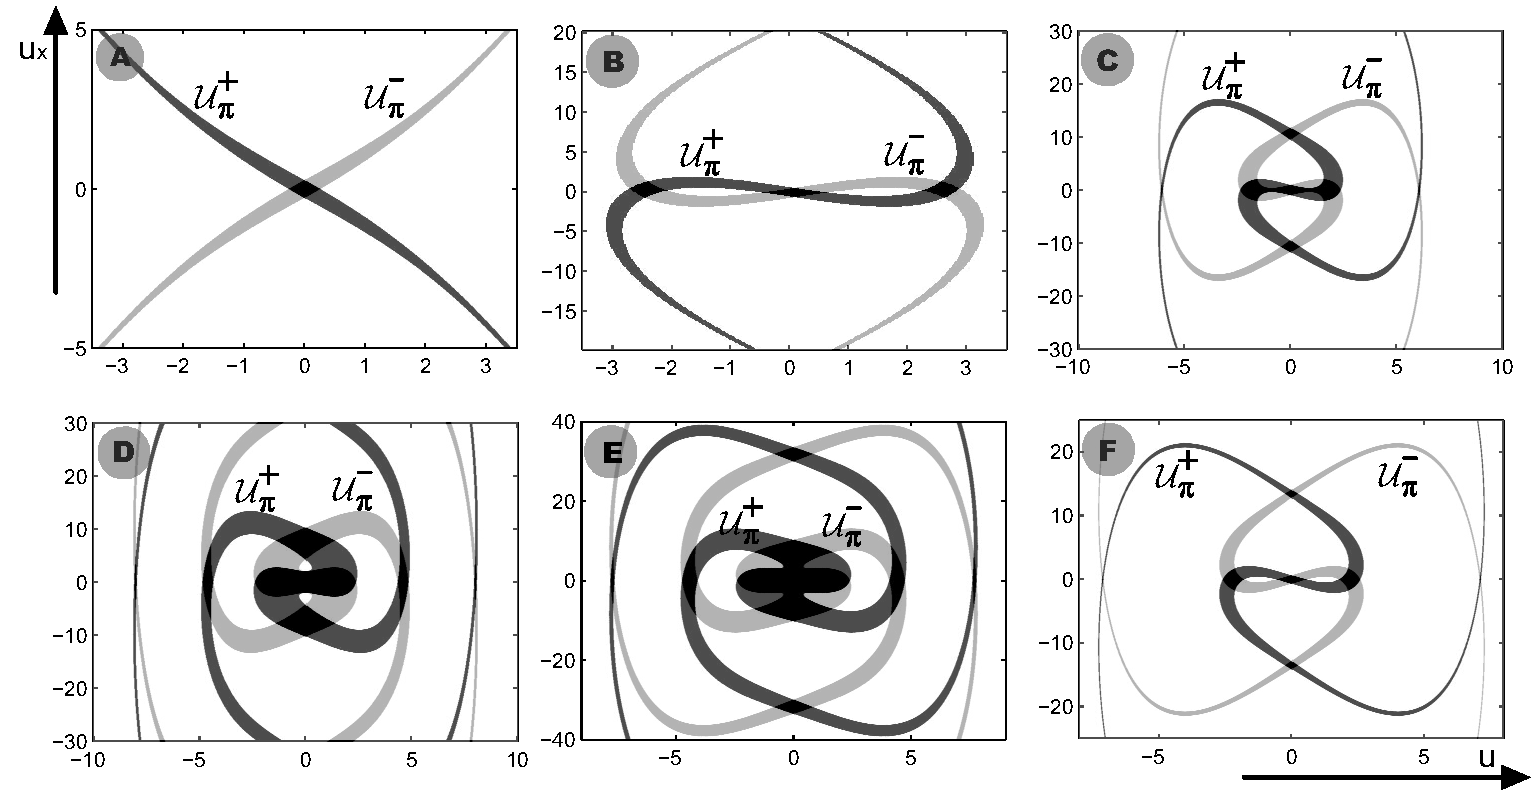
\includegraphics[width=0.8\textwidth]{pic/sets.pdf}
		\caption{Множества $\mathscr{U}_{\pi} = \mathscr{U}_{\pi}^+ \cap \mathscr{U}_{\pi}^-$ для различных значений $\omega$, $\alpha$.}
		\label{pic:sets}
	\end{figure}
\end{frame}

% ************
% * SLIDE 14 *
% ************
\begin{frame}
	\frametitle{Классификация}
	\framesubtitle{Построение алфавита: $\omega = -1$, $\alpha = -0.1$}
	\begin{figure}
		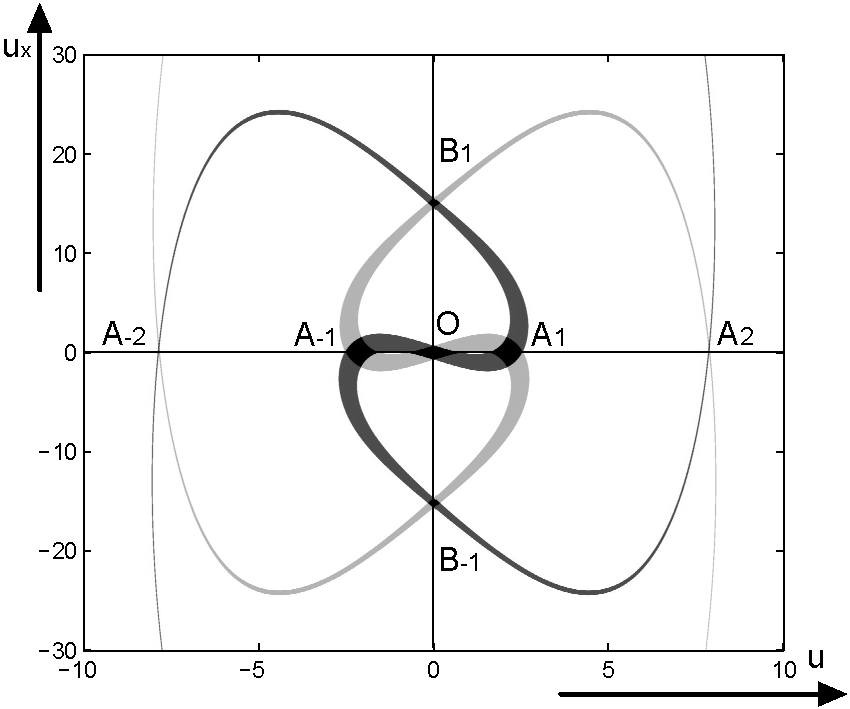
\includegraphics[width=0.65\textwidth]{pic/alphabet.pdf}
		\caption{Спиралевидная структура $\mathscr{U}_{\pi}^{\pm}$ $\Rightarrow$ бесконечный алфавит.}
		\label{pic:alphabet}
	\end{figure}
\end{frame}

% ************
% * SLIDE 15 *
% ************
\begin{frame}
	\frametitle{Классификация}
	\framesubtitle{Кодировка решений}
	
	\begin{figure}
		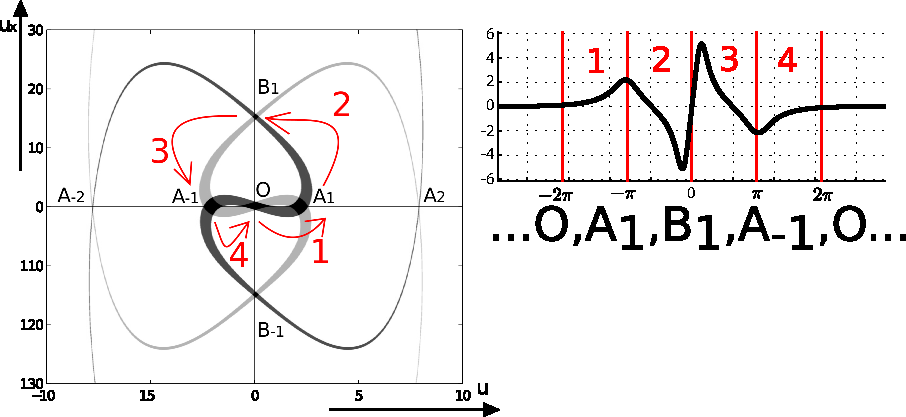
\includegraphics[width=1\textwidth]{pic/coding.pdf}
		\caption{Пример построение кода для заданного решения.}
		\label{pic:coding}
	\end{figure}
\end{frame}

% ************
% * SLIDE 16 *
% ************
\begin{frame}
	\frametitle{Классификация}
	\framesubtitle{Взаимно однозначное соответствие}
	
	Когда соответствие $\Sigma$ является взаимно однозначным?\footnotemark[3]
	\begin{enumerate}
		\item Множество $\mathscr{U}_L$ состоит из непересекающихся {\it островов}: $\mathscr{U}_L = \bigcup_{i \in S} D_i$.
		\item $\mathcal{P} D_i \cap D_j$, $\mathcal{P} D_i \cap D_j$ непусты; действие $\mathcal{P}$ на кривые внутри $D_i$ сохраняет свойства монотонности.
		\item $\Delta_0 = \mathscr{U}_L$, \quad $\Delta_{n + 1}^+ = \mathcal{P} \Delta_n^+ \cap \Delta_0$, \quad $\Delta_{n + 1}^- = \mathcal{P}^{-1} \Delta_n^- \cap \Delta_0$,\begin{center}
				$\lim \limits_{n \to \infty} \mu( \Delta_n^{\pm} ) = 0$.
			\end{center} 
	\end{enumerate}
	
	% Here could be some pictures, which clarify dynamics of the Poincare map on the phase plane.
	% Some h, v - strips could be depicted here.
	\begin{figure}
		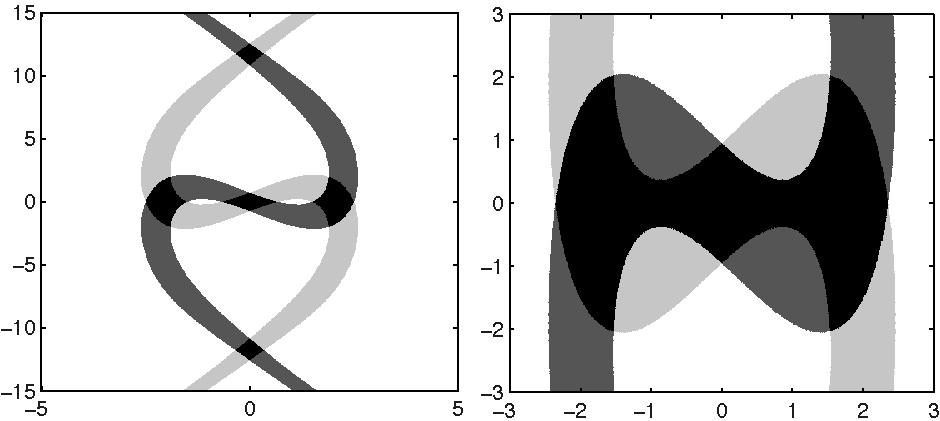
\includegraphics[width=0.5\textwidth]{pic/islands.pdf}
		\caption{Пример островного и не островного множества $\mathscr{U}_{L}$.}
		\label{pic:coding}
	\end{figure}
	
	\footnotetext[3]{\footnotesize{G. L. Alfimov, A. I. Avramenko, Physica D 254, 29 (2013)}}
\end{frame}

% ************
% * SLIDE 17 *
% ************
\begin{frame}	
	\begin{figure}
		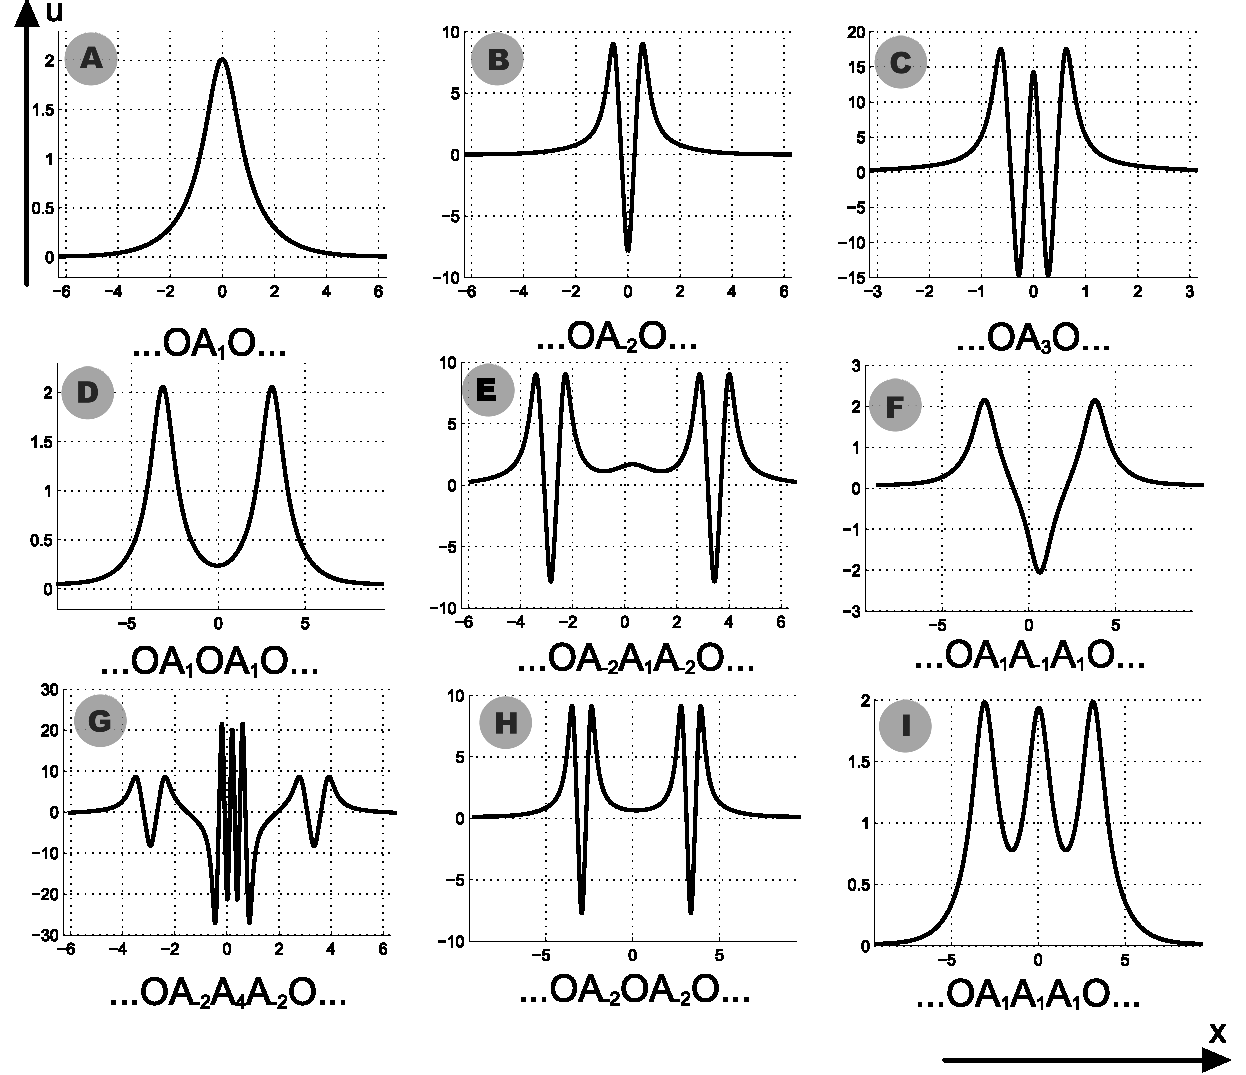
\includegraphics[width=0.8\textwidth]{pic/classification.pdf}
		\caption{Решения и их коды при $\omega = -1$, $\alpha = -0.1$.}
		\label{pic:classification}
	\end{figure}
\end{frame}

% ************
% * SLIDE 18 *
% ************
\begin{frame}
	\frametitle{Устойчивость}
	\framesubtitle{Аппарат\footnotemark[4]}
	
	% Copy Bogolyubov stability definition from Kizin presentation.
	Исходное уравнение:
	\begin{equation}
		i \Psi_t + \Psi_{xx} + F(|\Psi|^2, x) \Psi = 0.
		\label{eq:stability}
	\end{equation}

	Малые возмущения стационарного решения:
	\begin{equation}
		\Psi(t, x) = (u(x) + \widetilde{R}(t, x)) e^{-i \omega t}, \quad \widetilde{R} \ll 1.
		\label{eq:perturbation}
	\end{equation}
	
	Ищем решение в виде:
	\begin{equation}
		\widetilde{R}(t, x) = (a(x) + b(x)) e^{\lambda t} + (a^*(x) - b^*(x)) e^{\lambda^* t}.
		\label{eq:ansatz}
	\end{equation}
	
	Задача на собственные значения:
	\begin{equation}
		i \begin{pmatrix} 0 & \mathcal{L}_0 \\ \mathcal{L}_1 & 0 \end{pmatrix} \begin{pmatrix} a \\ b \end{pmatrix} = \lambda \begin{pmatrix} a \\ b \end{pmatrix};
		\label{eq:eigenvalues}
	\end{equation}
	\begin{eqnarray}
		&& \mathcal{L}_0 = \partial_{xx} + \omega + F(u^2, x); \\
		&& \mathcal{L}_1 = \partial_{xx} + \omega + F(u^2, x) + 2u^2 F_{|\Psi|^2}(u^2, x).
	\end{eqnarray}
	
	\footnotetext[4]{\footnotesize{Jianke Yang, Nonlinear Waves in Integrable and Nonintegrable Systems // Society of Industrial and Applied Mathematics (2010)}}
\end{frame}

% ************
% * SLIDE 19 *
% ************
\begin{frame}
	\frametitle{Устойчивость}
	\framesubtitle{Метод коллокаций Фурье}
	
	Рассматриваем локализованное решение на отрезке: $[-\frac{M}{2}; \frac{M}{2}]$.
	
	Ищем решение задачи \eqref{eq:eigenvalues} в виде разложений в ряды Фурье:
	\begin{equation}
		a(x) = \sum \limits_{n \in \mathbb{Z}} a_n e^{i \frac{2 \pi n}{M} x}, \quad b(x) = \sum \limits_{n \in \mathbb{Z}} b_n e^{i \frac{2 \pi n}{M} x}.
		\label{eq:solutions_expansions}
	\end{equation}
	
	Соответствующие представления для операторов $\mathcal{L}_0$, $\mathcal{L}_1$:
	\begin{equation}
		\mathcal{L}_0 = \partial_{xx} + \sum \limits_{n \in \mathbb{Z}} c_n^{(0)} e^{i \frac{2 \pi n}{M} x}, \quad \mathcal{L}_1 = \partial_{xx} + \sum \limits_{n \in \mathbb{Z}} c_n^{(1)} e^{i \frac{2 \pi n}{M} x}.
		\label{eq:operators_expansions}
	\end{equation}
	
	Подставляя \eqref{eq:solutions_expansions}, \eqref{eq:operators_expansions} в \eqref{eq:eigenvalues}, получаем систему линейных уравнений:
	\begin{equation}
		\begin{cases}
			-i \lambda a_k = -b_k (k k_0)^2 + \sum \limits_{n \in \mathbb{Z}} c_n^{(0)} b_{k - n} \\
			-i \lambda b_k = i a_k (k k_0)^2 + i \sum \limits_{n \in \mathbb{Z}} c_n^{(1)} a_{k - n} \\
		\end{cases}, \quad k \in \mathbb{Z}.
		\label{eq:system}
	\end{equation}
	
	Ограничим количество гармоник Фурье: $k \in [-K; K]$ $\Rightarrow$ задача на собственные значения оператора конечной размерности.
\end{frame}

% ************
% * SLIDE ?? *
% ************
%\begin{frame}
%	\frametitle{Устойчивость}
%	\framesubtitle{Недостатки подхода}
%	Осцилляторная неустойчивость, функция Эванса.
%\end{frame}

% ************
% * SLIDE 20 *
% ************
\begin{frame}
	\frametitle{Устойчивость}
	\framesubtitle{Тест}
	
	\begin{enumerate}
		\item[(A)] Решение $|\Psi(t, x)|$ {\it {\color{forestgreen} линейно устойчиво}}: весь спектр $\{ \lambda_i \}$ является мнимым.
		\item[(B)] Решение $|\Psi(t, x)|$ {\it {\color{fireenginered} экспоненциально неустойчиво}}: $\exists$ пара действительных собственных значений $\pm \lambda$.
		\item[(C)] Решение $|\Psi(t, x)|$ {\it {\color{fireenginered} осцилляторно неустойчиво}}: $\exists$ четверка комплексных собственных значений $\pm \lambda$, $\pm \lambda^*$.
	\end{enumerate}
	
	\begin{figure}
		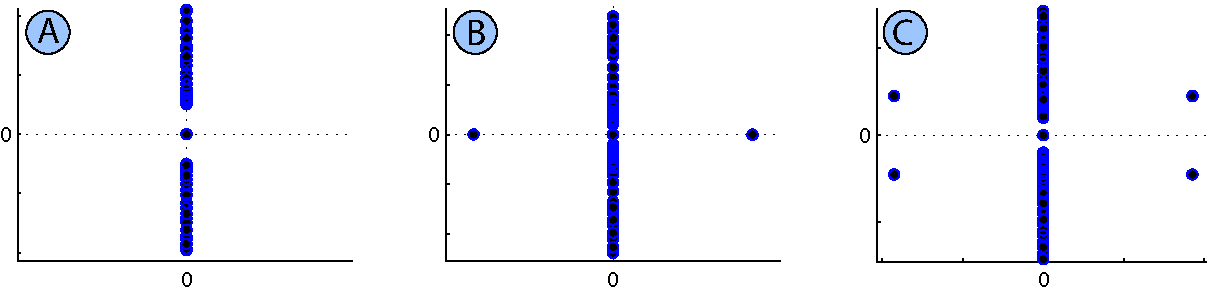
\includegraphics[width=0.8\textwidth]{pic/test.pdf}
		\caption{Примеры спектров для различных типов устойчивости.}
		\label{pic:test}
	\end{figure}
	
	Далее представлены результаты для:
	$$F(|\Psi|^2, x) = (\alpha + \cos 2x) |\Psi|^2.$$
\end{frame}

% ************
% * SLIDE 21 *
% ************
\begin{frame}
	\frametitle{Устойчивость}
	\framesubtitle{Примеры: фундаментальное решение}
	
	\begin{figure}
		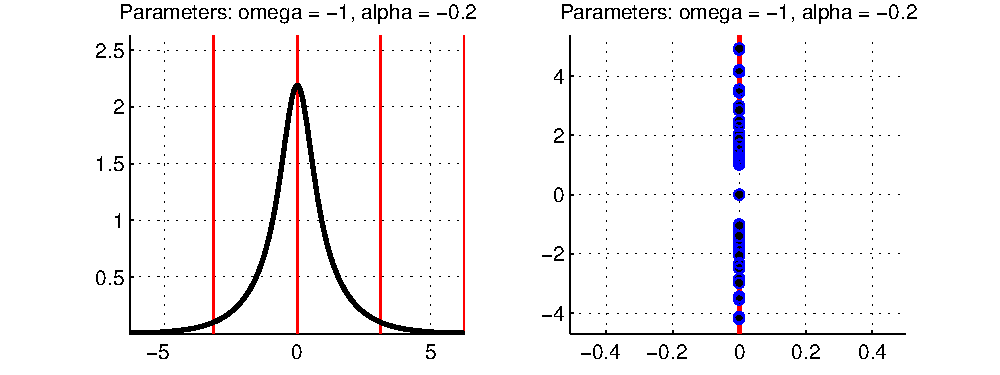
\includegraphics[width=1\textwidth]{pic/example_1.pdf}
		\caption{Фундаментальное решение $\dots O A_1 O \dots$, {\it \color{forestgreen}{линейно устойчиво}}.}
		\label{pic:example_1}
	\end{figure}
\end{frame}

% ************
% * SLIDE 22 *
% ************
\begin{frame}
	\frametitle{Устойчивость}
	\framesubtitle{Примеры: дипольное решение}
	
	\begin{figure}
		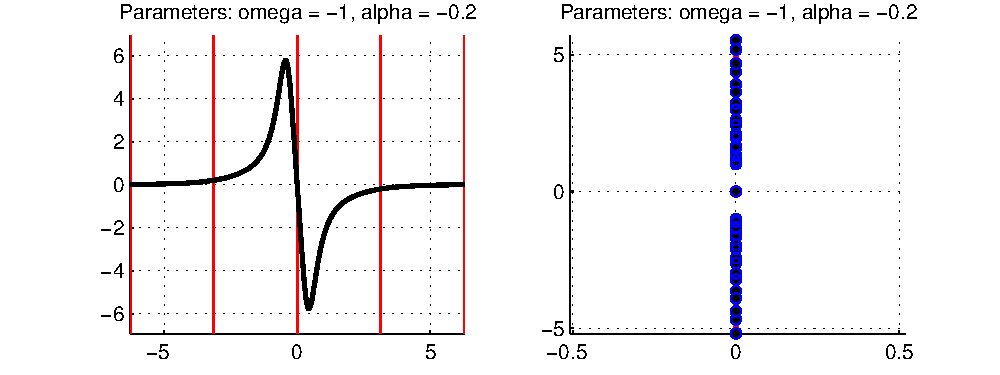
\includegraphics[width=1\textwidth]{pic/example_2.pdf}
		\caption{Дипольное решение $\dots O B_{-1} O \dots$, {\it \color{forestgreen}{линейно устойчиво}}.}
		\label{pic:example_2}
	\end{figure}
\end{frame}

% ************
% * SLIDE 23 *
% ************
\begin{frame}
	\frametitle{Устойчивость}
	\framesubtitle{Примеры}
	
	\begin{figure}
		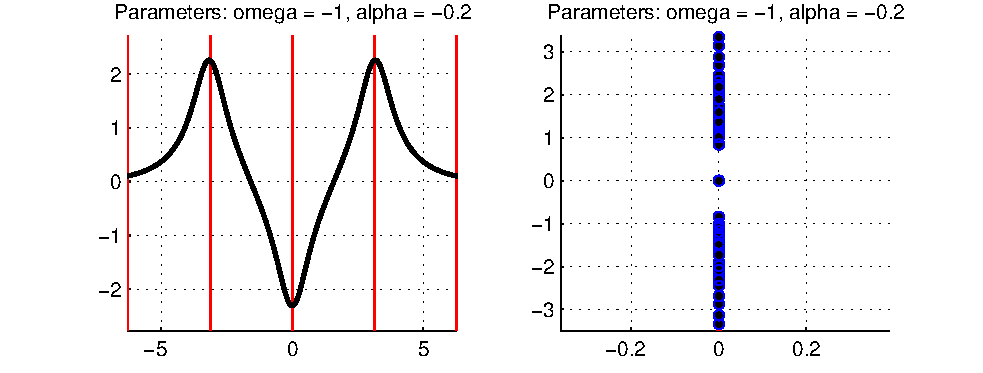
\includegraphics[width=1\textwidth]{pic/example_3.pdf}
		\caption{Решение $\dots O A_1 A_{-1} A_1 O \dots$, {\it \color{forestgreen}{линейно устойчиво}}.}
		\label{pic:example_3}
	\end{figure}
\end{frame}

% ************
% * SLIDE 24 *
% ************
\begin{frame}
	\frametitle{Устойчивость}
	\framesubtitle{Примеры}
	
	\begin{figure}
		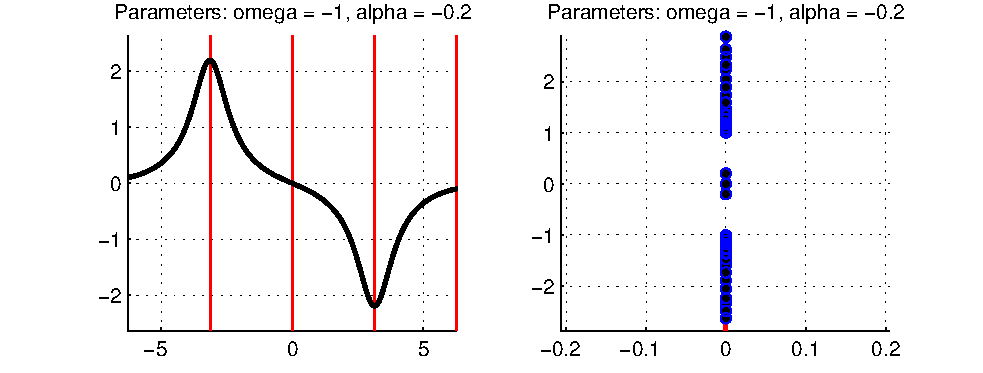
\includegraphics[width=1\textwidth]{pic/example_4.pdf}
		\caption{Решение $\dots O A_1 O A_{-1} O \dots$, {\it \color{forestgreen}{линейно устойчиво}}.}
		\label{pic:example_4}
	\end{figure}
\end{frame}

% ************
% * SLIDE 25 *
% ************
\begin{frame}
	\frametitle{Устойчивость}
	\framesubtitle{Примеры}
	
	\begin{figure}
		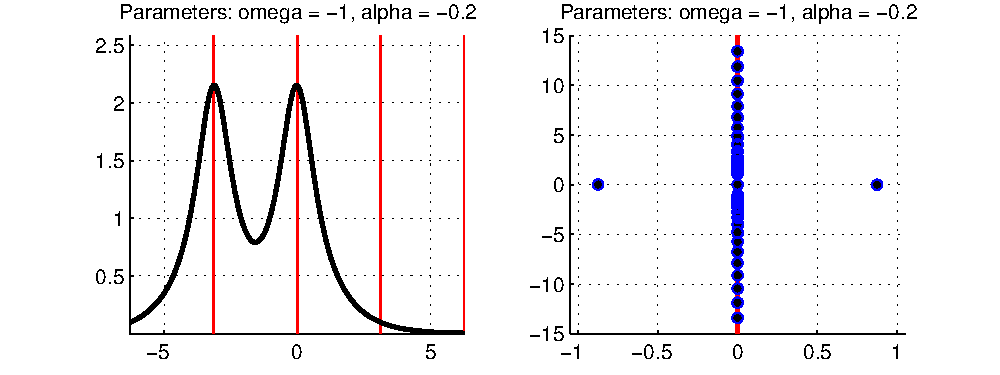
\includegraphics[width=1\textwidth]{pic/example_5.pdf}
		\caption{Решение $\dots O A_1 A_1 O \dots$, {\it \color{fireenginered}{экспоненциально неустойчиво}}.}
		\label{pic:example_5}
	\end{figure}
\end{frame}

% ************
% * SLIDE 26 *
% ************
\begin{frame}
	\frametitle{Устойчивость}
	\framesubtitle{Примеры}
	
	\begin{figure}
		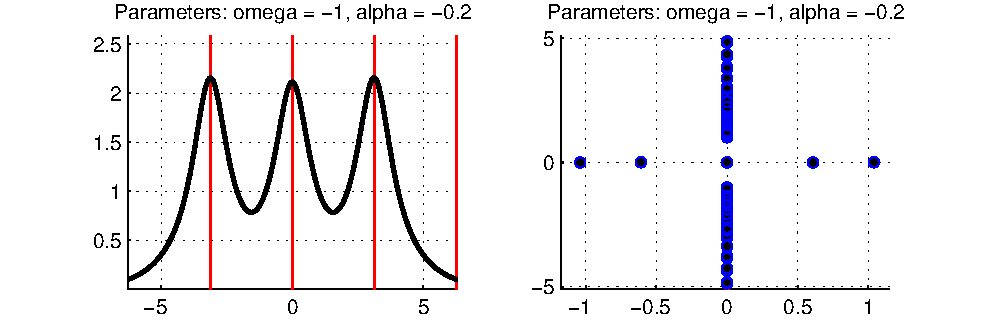
\includegraphics[width=1\textwidth]{pic/example_6.pdf}
		\caption{Решение: $\dots O A_1 A_1 A_1 O \dots$, {\it \color{fireenginered}{экспоненциально неустойчиво}}.}
		\label{pic:example_6}
	\end{figure}
\end{frame}

% ************
% * SLIDE 27 *
% ************
\begin{frame}
	\frametitle{Устойчивость}
	\framesubtitle{Примеры}
	
	\begin{figure}
		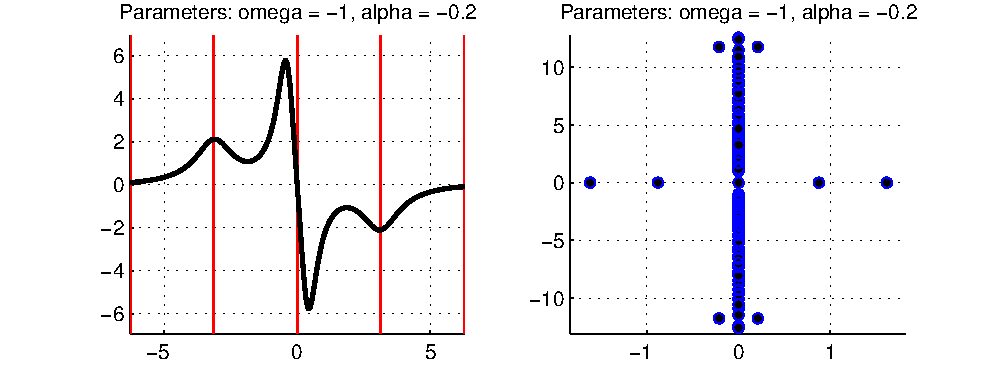
\includegraphics[width=1\textwidth]{pic/example_7.pdf}
		\caption{Решение: $\dots O A_1 B_{-1} A_{-1} O \dots$, {\it \color{fireenginered}{экспоненциально неустойчиво}}.}
		\label{pic:example_7}
	\end{figure}
\end{frame}

% ************
% * SLIDE 28 *
% ************
\begin{frame}
	\frametitle{Устойчивость}
	\framesubtitle{Примеры}
	
	\begin{figure}
		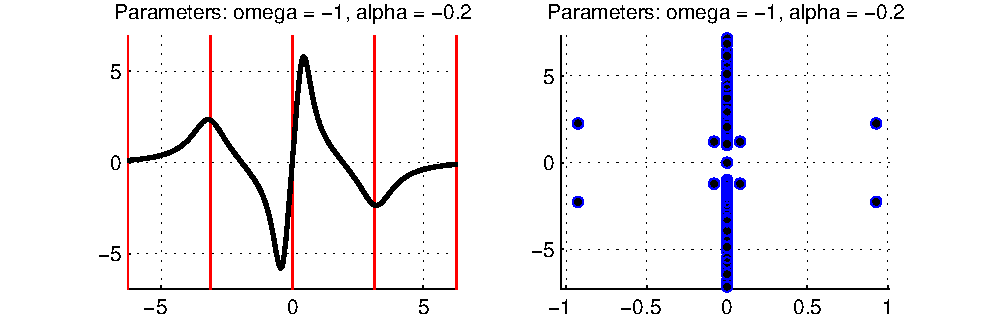
\includegraphics[width=1\textwidth]{pic/example_8.pdf}
		\caption{Решение: $\dots O A_1 B_1 A_{-1} O \dots$, {\it \color{fireenginered}{осцилляторно неустойчиво}}.}
		\label{pic:example_8}
	\end{figure}
\end{frame}

% ************
% * SLIDE 29 *
% ************
\begin{frame}
	\frametitle{Устойчивость}
	\framesubtitle{Результаты}
	
	\begin{equation}
		i \Psi_t + \Psi_{xx} + (\alpha + \cos 2x) |\Psi|^2 \Psi = 0
		\label{eq:results}	
	\end{equation}
	
	\begin{itemize}
		\item Множество стационарных решений уравнения \eqref{eq:results} чрезвычайно богато.
		\item Большинство стационарных решений оказываются неустойчивы; исключение составляют:
			\begin{enumerate}
				\item[1.] Фундаментальное решение: $\dots O A_{\pm 1} O \dots$.
				\item[2.] Дипольное решение: $\dots O B_{\pm 1} O \dots$ ({\bf {\color{red} new}}).
				\item[3.] Некоторые комбинации {\color{ceruleanblue} (1)} и {\color{ceruleanblue} (2)}: $\dots O A_1 A_{-1} A_1 O \dots$, $\dots O A_1 O A_{-1} O \dots$.
			\end{enumerate}
	\end{itemize}
\end{frame}

% ************
% * SLIDE 30 *
% ************
\begin{frame}
	\frametitle{Устойчивость}
	\framesubtitle{Расчёт эволюции}
	
	Для расчёта используем консервативную разностную схему Сухорукова\footnotemark[6].
	Она сохраняет два интеграла:
	\begin{equation}
		N(t) = \int |\Psi(t, x)|^2 dx; \quad
		E(t) = \dfrac{1}{2} \int \Psi^*(t, x) \widehat{H} \Psi(t, x) dx
	\end{equation}

	Для подавления эффекта отражения излучения от краев области интегрирования при расчете, в схему добавлен {\it {\color{ceruleanblue} поглощающий слой}}. 
	
	\footnotetext[6]{\footnotesize{V. A. Trofimov, N. V. Peskov // Mathematical Modelling and Analysis, Volume 14 Number 1, 2009, pages 109-126}}
\end{frame}

% ************
% * SLIDE 31 *
% ************
\begin{frame}
	\frametitle{Устойчивость}
	\framesubtitle{Расчёт эволюции: дипольное решение}
	
	\begin{figure}
		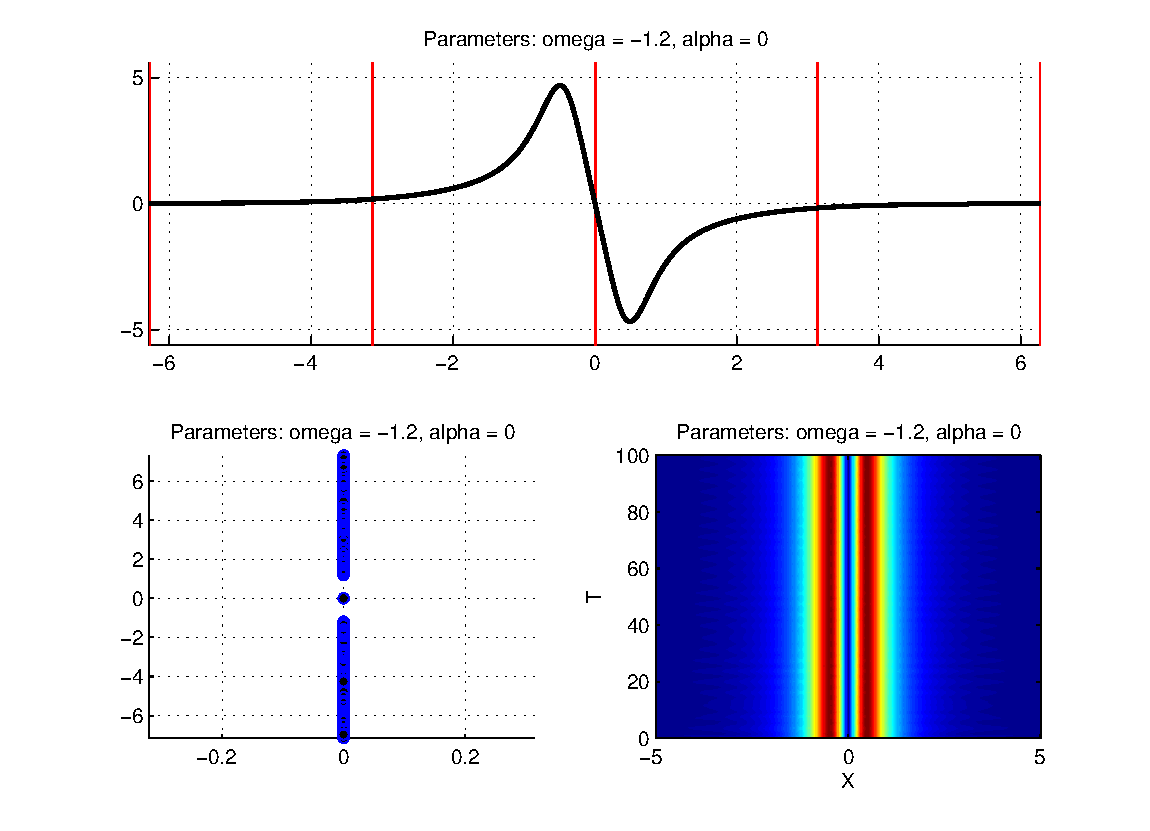
\includegraphics[width=0.8\textwidth]{pic/dipole_solution_stable.pdf}
		\caption{Устойчивое дипольное решение.}
		\label{pic:dipole_solution_stable}
	\end{figure}
\end{frame}

% ************
% * SLIDE 32 *
% ************
\begin{frame}
	\frametitle{Устойчивость}
	\framesubtitle{Расчёт эволюции: дипольное решение}
	
	\begin{figure}
		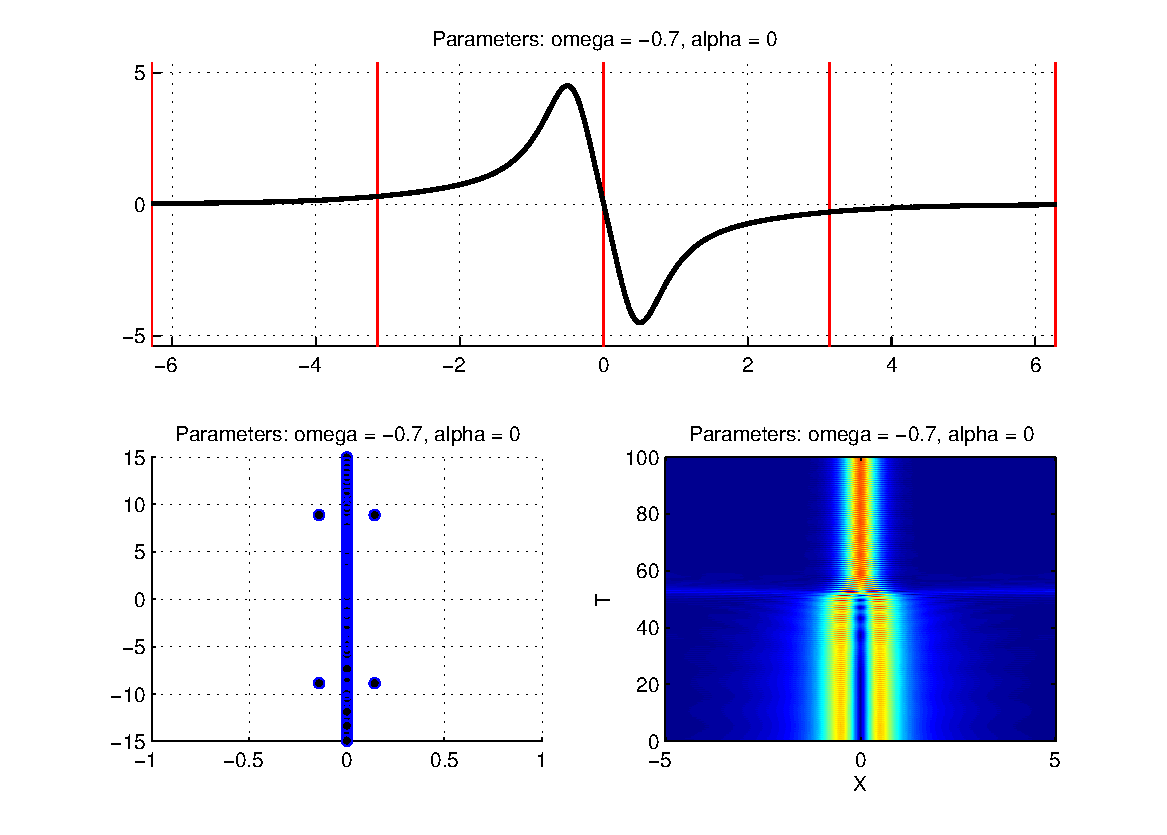
\includegraphics[width=0.8\textwidth]{pic/dipole_solution_unstable.pdf}
		\caption{Неустойчивое дипольное решение.}
		\label{pic:dipole_solution_unstable}
	\end{figure}
\end{frame}

% ************
% * SLIDE 33 *
% ************
\begin{frame}
	\begin{center}
		{\LARGE 3. Стационарные локализованные решения УГП в случае параболической потенциальной ямы и периодического псевдопотенциала, $$U(x) = x^2, \quad P(x) <> 0$$}
	\end{center}
\end{frame}

% ************
% * SLIDE 34 *
% ************
\begin{frame}
	\frametitle{Параболическая потенциальная яма}
	\framesubtitle{Простейший псевдопотенциал\footnotemark[7]}
	
	\begin{equation}
		i \Psi_t + \Psi_{xx} - x^2 \Psi \pm |\Psi|^2 \Psi = 0.
	\end{equation}
	
	Все локализованные решения имеют {\it \uwave{линейный аналог}}.
	
	\begin{figure}
		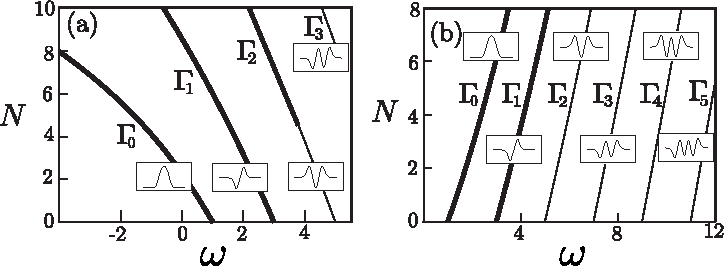
\includegraphics[width=0.9\textwidth]{pic/solution_branches_simple.pdf}
		\caption{Ветви различных локализованных решений и их устойчивость для случаев {\color{ceruleanblue} (a)} $P(x) \equiv +1$; {\color{ceruleanblue} (b)} $P(x) \equiv -1$.}
		\label{pic:branches_simple}
	\end{figure}
	
	\footnotetext[7]{\footnotesize{D. A. Zezyulin, G. L. Alfimov, V. V. Konotop and V. M. P\'erez-Garcia // Phys. Rev. A {\bf 76}, 013621 (2007)}}
\end{frame}

% ************
% * SLIDE 35 *
% ************
\begin{frame}
	\frametitle{Параболическая потенциальная яма}
	\framesubtitle{Периодический псевдопотенциал с ненулевым средним}
	
	\begin{equation}
		i \Psi_t + \Psi_{xx} - x^2 \Psi + (1 + \beta \cos \Omega x) |\Psi|^2 \Psi = 0.
	\end{equation}

	Появляются решения, {\it не имеющие линейного аналога}.

	\begin{figure}
		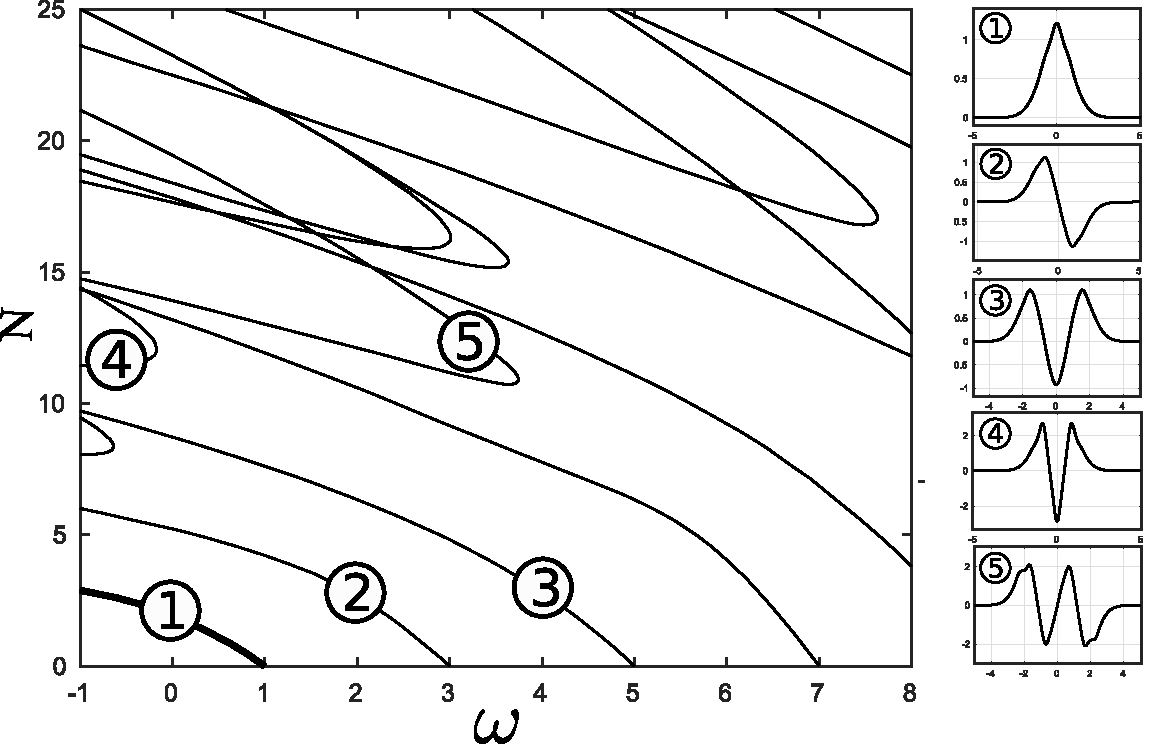
\includegraphics[width=0.65\textwidth]{pic/solution_branches_nonzero_mean.pdf}
		\caption{Ветви различных локализованный решений и их устойчивость для $\beta = 2$, $\Omega = 8$.}
		\label{pic:branches_nonzero_mean}
	\end{figure}	
	
\end{frame}

% ************
% * SLIDE 36 *
% ************
\begin{frame}
	\frametitle{Параболическая потенциальная яма}
	\framesubtitle{Периодический псевдопотенциал с нулевым средним}
	
	\begin{equation}
		i \Psi_t + \Psi_{xx} - x^2 \Psi + \cos \Omega x |\Psi|^2 \Psi = 0.
	\end{equation}

	Ветвь решения {\color{ceruleanblue} (1)} устойчива при $\omega \approx 5$.

	\begin{figure}
		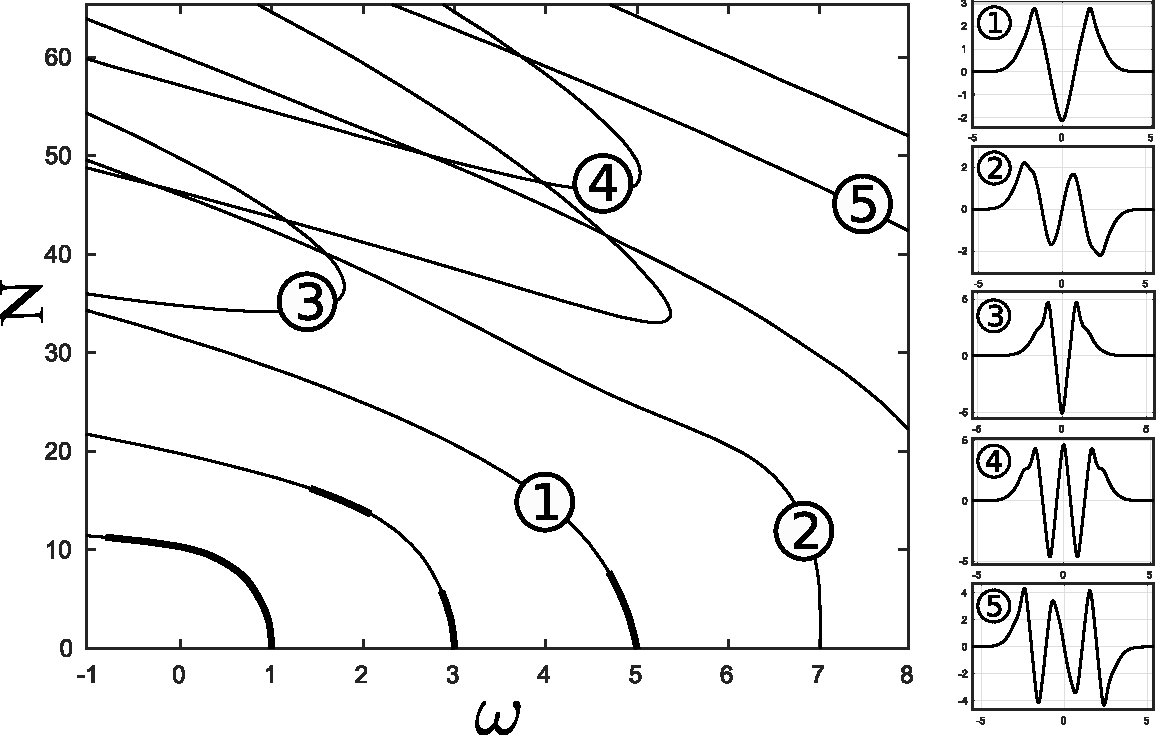
\includegraphics[width=0.65\textwidth]{pic/solution_branches_zero_mean.pdf}
		\caption{Ветви различных локализованный решений и их устойчивость для $\Omega = 8$.}
		\label{pic:branches_zero_mean}
	\end{figure}	
	
\end{frame}

% ************
% * SLIDE 37 *
% ************
\begin{frame}
	\frametitle{Предельный переход $\Omega \to +\infty$}
	\framesubtitle{Периодический псевдопотенциал с ненулевым средним}
	
	\begin{figure}
		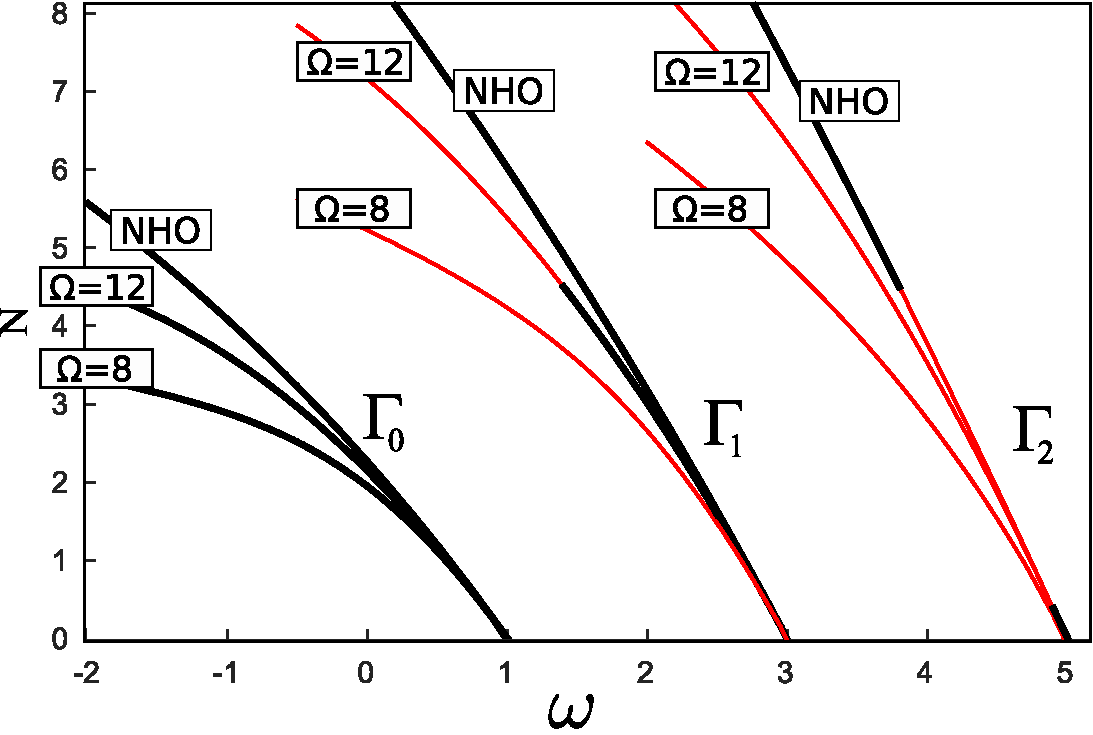
\includegraphics[width=0.8\textwidth]{pic/nonlinear_oscillator_limit.pdf}
		\caption{Переход к нелинейному гармоническому осциллятору при $\Omega \to +\infty$ для $P(x) = 1 + \cos \Omega x$.}
		\label{pic:nonlinear_limit}
	\end{figure}	
\end{frame}

% ************
% * SLIDE 38 *
% ************
\begin{frame}
	\frametitle{Предельный переход $\Omega \to +\infty$}
	\framesubtitle{Периодический псевдопотенциал с нулевым средним}
	
	\begin{figure}
		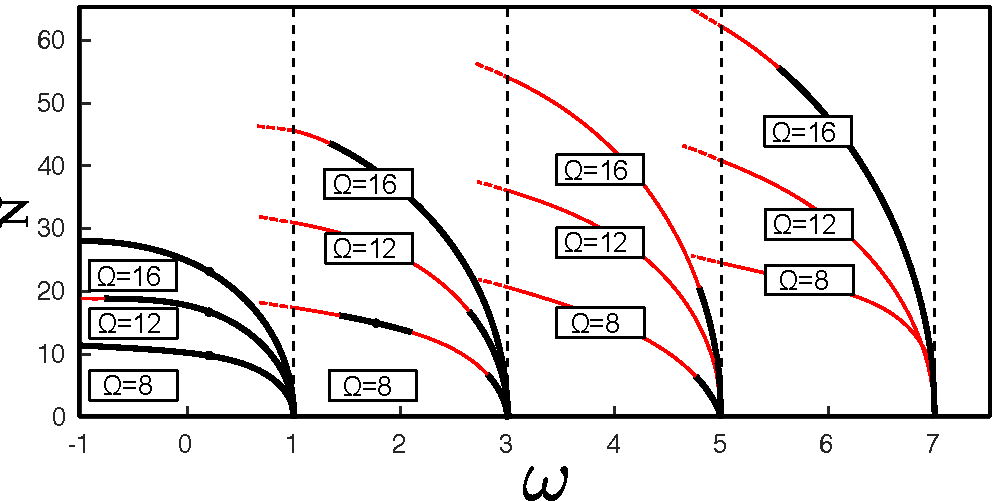
\includegraphics[width=0.8\textwidth]{pic/linear_oscillator_limit.pdf}
		\caption{Переход к линейному гармоническому осциллятору при $\Omega \to +\infty$ для $P(x) = \cos \Omega x$.}
		\label{pic:linear_limit}
	\end{figure}
\end{frame}

% ************
% * SLIDE 39 *
% ************
\begin{frame}
	\frametitle{Потеря устойчивости решений с линейным аналогом}
	
	\begin{figure}
		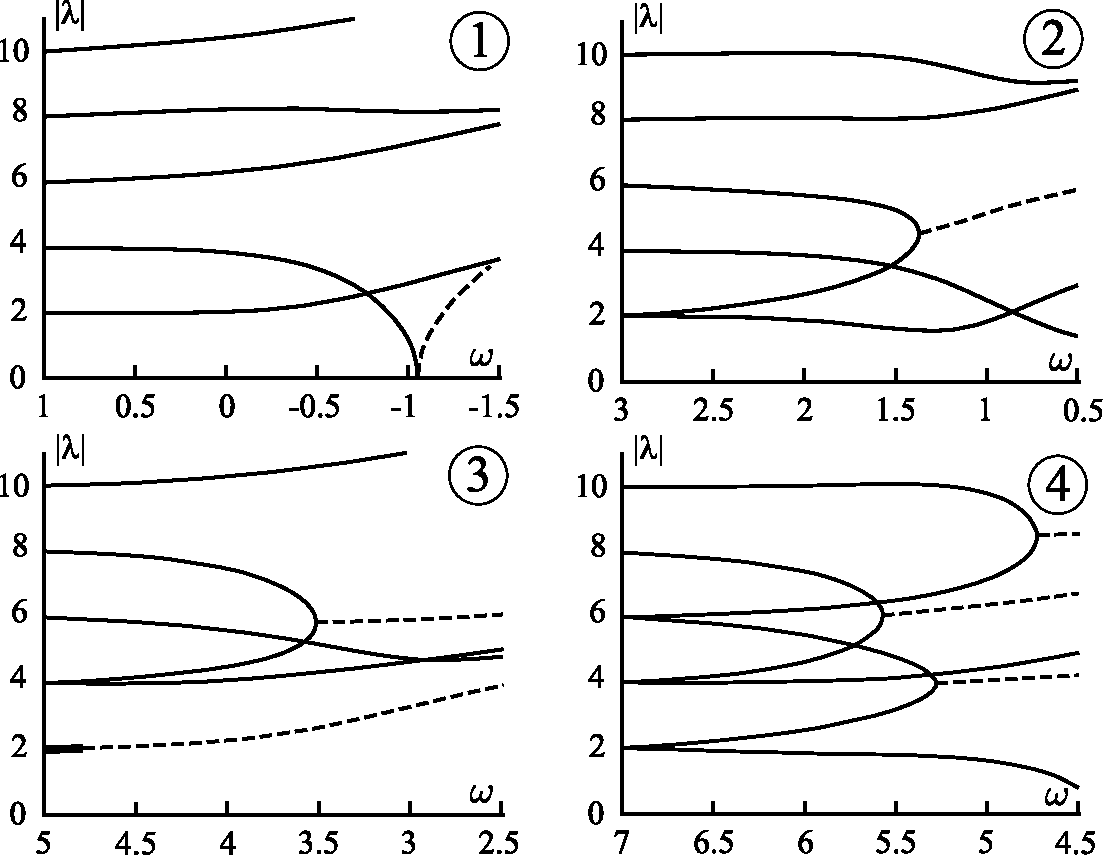
\includegraphics[width=0.75\textwidth]{pic/stability_loss.pdf}
		\caption{Сценарии потери устойчивости первых четырёх ветвей  решений с линейным аналогом для $P(x) = \cos 16 x$.}
		\label{pic:stability_loss}
	\end{figure}
\end{frame}

% ************
% * SLIDE ?? *
% ************
%\begin{frame}
%	\frametitle{Сценарий потери устойчивости}
%	\framesubtitle{Асимптотическое приближение}
%\end{frame}

% ************
% * SLIDE 40 *
% ************
\begin{frame}
	\frametitle{Классическая потенциальная яма}
	\framesubtitle{Расчёт эволюции}
	
	\begin{figure}
		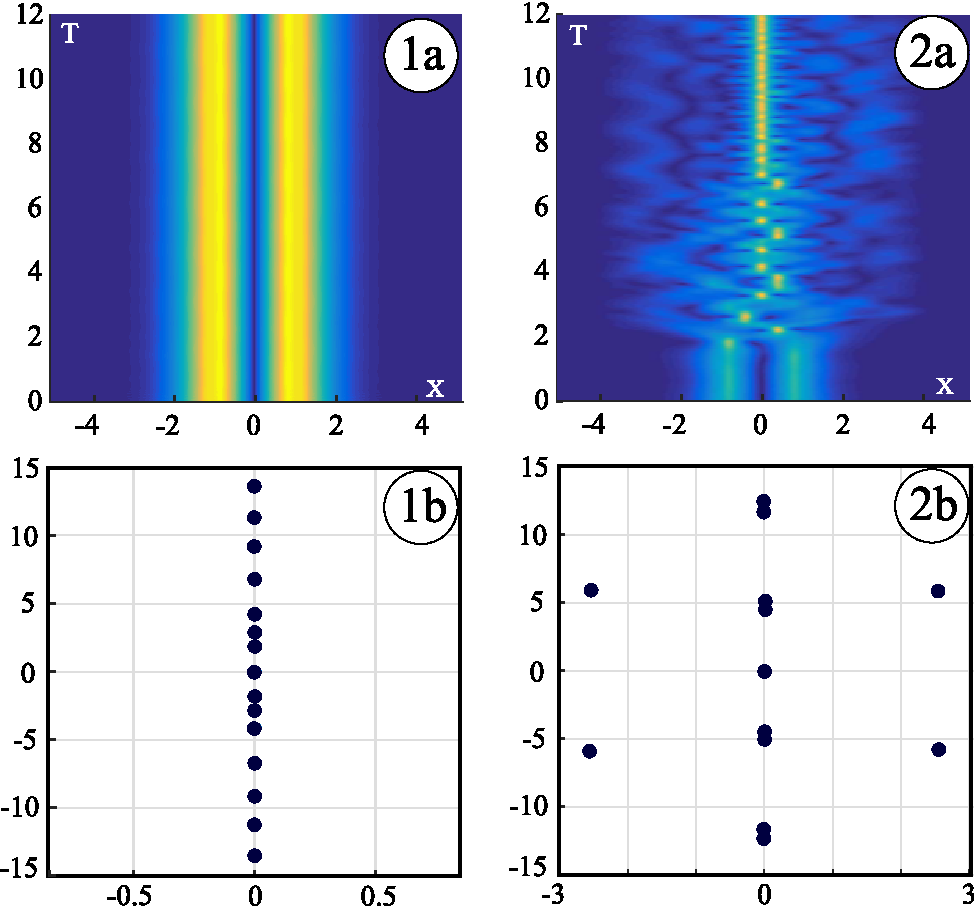
\includegraphics[width=0.6\textwidth]{pic/evolution.pdf}
		\caption{Решение $\Gamma_1$ при $P(x) = \cos 16 x$ для {\color{ceruleanblue} (1)} $\omega = 2$ и {\color{ceruleanblue} (2)} $\omega = 0$.}
		\label{pic:evolution}
	\end{figure}
\end{frame}

% ************
% * SLIDE 41 *
% ************
\begin{frame}
	\frametitle{Классическая потенциальная яма}
	\framesubtitle{Результаты}
	
	\begin{itemize}
		\item Присутствие периодического псевдопотенциала приводит к появлению локализованных решений без линейного аналога.
		\item В предельном случае $\Omega \to +\infty$ задача приближается к линейному или нелинейному гармоническому осциллятору.
		\item Сценарий потери устойчивости для решений с линейным аналогом ({\it {\color{ceruleanblue} исследован асимптотически и численно}}):
		\begin{enumerate}
			\item При $P(x) = 0$ некоторые $\lambda_i$ удвоены.
			\item Удвоенные $\lambda_i$ расщепляются под действием возмущения $P(x) \neq 0$.
			\item При расщеплении могут образовывать $\lambda_i$ с ненулевой действительной частью.
		\end{enumerate}
	\end{itemize}
\end{frame}

% ************
% * SLIDE XX *
% ************
%\begin{frame}
%	\frametitle{Содержание}
%	\tableofcontents
%\end{frame}

% ************
% * SLIDE 42 *
% ************
\begin{frame}
	\frametitle{Основные результаты и положения}
	\framesubtitle{выносимые на защиту}

	\begin{small}
	\begin{itemize}
		\setlength\itemsep{10pt}
		\item[1.] Сформулированы достаточные условия, гарантирующие {\color{ceruleanblue} (а)} наличие и {\color{ceruleanblue} (б)} отсутствие сингулярных решений стационарного УГП.
		Доказаны утверждения о существовании семейств сингулярных решений, соответствующих случаю ``общего положения''.
		\item[2.] Предложен метод описания стационарных локализованных решений УГП с нулевым потенциалом и периодическим псевдопотенциалом в терминах символической динамики.
		Использование этого метода позволило обнаружить новое устойчивое решение УГП, т.н. дипольное локализованной решение, а также ряд устойчивых связанных состояний.
		\item[3.] Показано, что наличие периодического псевдопотенциала высокой частоты позволяет стабилизировать неустойчивые нелинейные локализованные решения, существующие в модели УГП с квадратичным потенциалом.
	\end{itemize}	
	\end{small}	
\end{frame}

% ************
% * SLIDE 43 *
% ************
\begin{frame}
	\frametitle{Публикации}
	
	\begin{large}
	{
		\color{ceruleanblue}
		11 публикаций, \\
		3 статьи, индексируемые системой Scopus.
	}	
	\end{large}

	\medskip

	% Rework with some bibliography style approach.
	\begin{scriptsize}
	\begin{enumerate}
		\setlength\itemsep{10pt}
		\item[1.] Алфимов Г. Л., Лебедев М. Е., О регулярных и сингулярных решениях уравнения $u_{xx} + Q(x) u + P(x) u^3 = 0$ // Уфимск. матем. журн. том {\bf 7}, выпуск 2, стр. 3--18 (2015).
		\item[2.] Lebedev M. E., Alfimov G. L., Malomed B. A., Stable dipole solitons and soliton complexes in the nonlinear Schr\"odinger equation with periodically modulated nonlinearity // Chaos: An Interdisciplinary Journal of Nonlinear Science {\bf 26} (7), 073110 (2016)
		\item[3.] Alfimov G. L., Gegel L. A., Lebedev M. E., Malomed B. A., Zezyulin D. A., Localized modes in the Gross-Pitaevskii equation with a parabolic trapping potential and a nonlinear lattice pseudopotential // Communications in Nonlinear Science and Numerical Simulation {\bf 66}, 194-207 (2019).
		\item[5.] Alfimov G. L., Lebedev M. E., Coding of stationary modes for the nonlinear Schr\"odinger equation with periodically modulated nonlinearity // Мат. конф. ``Hamiltonian Dynamics, Nonautonomous Systems, and Patterns in PDE’s'', НГУ, Нижний Новгород, декабрь 2014.
		\item[6.] Алфимов Г. Л., Лебедев М. Е., Стационарные моды нелинейного уравнения Шрёдингера в присутствии линейного и нелинейного потенциалов // Мат. конф. ``Фундаментальная математика и ее приложения в естествознании'', БашГУ, Уфа, сентябрь 2015.
	\end{enumerate}
	\end{scriptsize}
\end{frame}

\begin{frame}
	\frametitle{Публикации}
	
	\begin{scriptsize}	
	\begin{enumerate}
	\setlength\itemsep{10pt}
		\item[7.] Lebedev M. E., Alfimov G. L., Malomed B. A., Stable dipole solitons and soliton complexes in the nonlinear Schr\"odinger equation with periodically modulated nonlinearity // Мат. конф. ``Hamiltonian Dynamics, Nonautonomous Systems, and Patterns in PDE’s'', НГУ, Нижний Новгород, декабрь 2016.
		\item[8.] Alfimov G. L., Gegel L. A., Lebedev M. E., Zezyulin D. A., Malomed B. A., Steady-states for the Gross-Pitaevskii equation with nonlinear lattice pseudopotential // Мат. конф. `` Комплексный анализ, математическая физика и нелинейные уравнения'', озеро Банное, Башкортостан, март 2018.
		\item[9.] Alfimov G. L., Lebedev M. E., Zezyulin D. A., Malomed B. A., Steady-states for the Gross-Pitaevskii equation with nonlinear lattice pseudopotential // Конф. ``Nonlinear Phenomena in Bose Condensates and Optical Systems'', Ташкент, Узбекистан, август 2018.
		\item[10.] Zezyulin D. A., Lebedev M. E., Alfimov G. L., Malomed B. A., Symmetry breaking in competing single-well linear-nonlinear potentials // Мат. конф. `` Комплексный анализ, математическая физика и нелинейные уравнения'', озеро Банное, Башкортостан, март 2018.
		\item[11.] Lebedev M. E., Shipitsyn K. V., Codding of solutions for the Duffing equation with non-homogeneous nonlinearity // Мат. конф. `` Комплексный анализ, математическая физика и нелинейные уравнения'', озеро Банное, Башкортостан, март 2018.
	\end{enumerate}
	\end{scriptsize}
\end{frame}

% ************
% * SLIDE 43 *
% ************
\begin{frame}
	\begin{center}
		{\Huge Спасибо за внимание!}
	\end{center}
\end{frame}

\end{document} 